\section{Product}

This chapter gives a high level overview of the product. Paragraph 2.1 gives a brief analysis of the program and high level overview of the product backlog. In paragraph 2.2 the steps needed to create this program will be described in a roadmap of major releases. Here the major releases of the program are given in a clear overview.

\subsection{Program Overview}

\textbf{Analysis context} \\
Aircraft and airport noise are complex subject matters which have been studied for decades and are still the focus of many research efforts nowadays. Also at the department of Air Transport \& Operations (ATO) at TU Delft’s Faculty of Aerospace Engineering. ATO has three research aims: 1) To develop radical new ways to optimise aircraft operations for efficiency, safety, cost and environmental impact; 2) To extend the analysis to an airline fleet and network level to include capacity and resilience; 3) To synthesize these to include operational safety at an airline and ATM level. To support their research findings at conferences, they need a visualization application that does this.

\textbf{Analysis problem} \\
The ATO research department needs a program that represents a creative and efficient way to optimize and visualize aircraft noise along simulated and real flight routes. This requires the implementation of a mathematical model for aircraft noise and aircraft trajectory design. The model will be deployed by the research team to predict aircraft noise along a particular trajectory (flight route) in order to be able to optimize the trajectory and to reduce the produced noise. In order to implement this model the parameters that are required for the sound calculation need to be derived mathematically. Besides that, the program should also be able to visualize the noise produced along the simulated trajectory pictured on a real map. This requires an implementation of noise contours, which are ‘noise footprints’ whose shape indicate areas of constant noise. Noise contours are a new subject to the research group and haven’t been implemented in relation with trajectory optimization before so this will be a challenging topic. The visualization should also show the effects of the produced aircraft noise on population annoyance.

\textbf{Analysis stakeholder inputs} \\
The application needs to be able to read in two arbitrary data (.dat extension) or text files indicating the input trajectory (including selected airplane model) and the grid that needs to be used. These files will be given as input to the sound model. The sound model will then calculate the noise levels produced along the trajectory and the output of the sound model will be entered into the optimization model or will directly be sent to the visualization component.

Additionally, the stakeholder will deliver us some papers and extra explanation on the mathematical concepts behind the optimization model and contouring algorithm.

\textbf{Product backlog} \\
Our product should be able to do the following tasks:

\begin{itemize}
\item Optimize the existing sound model with multi-core processing to achieve real-time performance.
\item Calculate and output the actual noise contours produced along the input trajectory
\item Optimize the input trajectory based in order to reduce the produced noise 
\item Visualize the optimized trajectory together with the noise contours in real-time 3D animation mapped on Google Earth
\item Calculate and visualize the effects of produced noise on population annoyance using the awakenings algorithm
\item Save the results in a particular format and directory specified by the user
\item It should be possible to perform all these tasks in a graphical user interface
\end{itemize}

\newpage 

\subsection{Roadmap}
In the roadmap below major releases of the program are spread across different phases of software development and they are given in a clear overview. \\

\begin{figure}[ht]
    \centering
    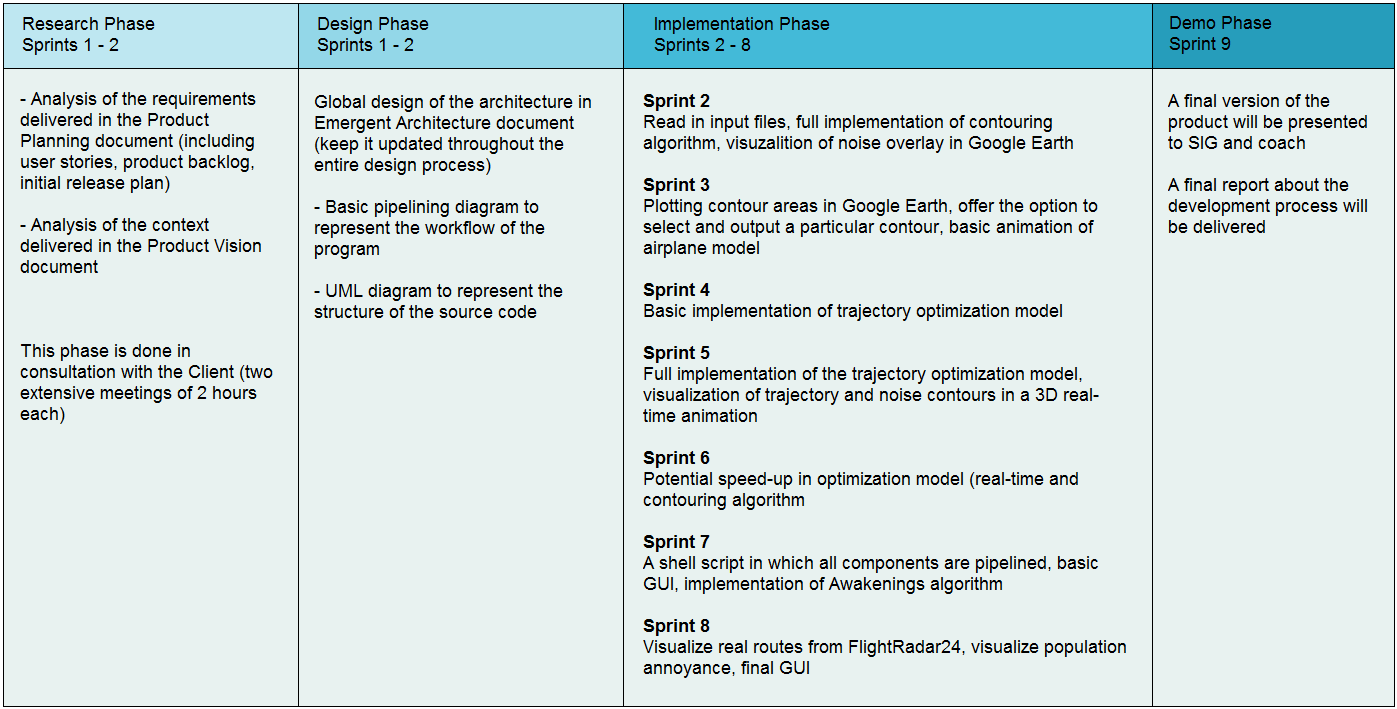
\includegraphics[width=1.1\textwidth]{images/roadmap}
\end{figure}